\documentclass[aspectratio=43, t]{beamer}
\usetheme{CSCS}

\usepackage{amsmath}
\usepackage{amssymb}
\usepackage{fontspec}
\usepackage{unicode-math}
\usepackage{pgfpages}
\usepackage{minted}
\usepackage{xurl}
\usepackage{hyperref}
\usepackage{booktabs}
\usepackage{multicol}
\usepackage{physics}
\usepackage{pgfplots}
\usepackage{tikzpagenodes}
\usetikzlibrary{arrows.meta}

\definecolor{ETH1}{cmyk/RGB/HTML}{1.00, 0.70, 0.00, 0.30 /  31,  64, 122 / 1F407A} % dark blue
\definecolor{ETH2}{cmyk/RGB/HTML}{0.75, 0.40, 1.00, 0.40 /  72,  90,  44 / 485A2C} % dark green
\definecolor{ETH3}{cmyk/RGB/HTML}{1.00, 0.50, 0.00, 0.00 /  18, 105, 176 / 1269B0} % blue
\definecolor{ETH4}{cmyk/RGB/HTML}{0.30, 0.00, 1.00, 0.55 / 114, 121,  28 / 72791C} % green
\definecolor{ETH5}{cmyk/RGB/HTML}{0.20, 1.00, 0.00, 0.20 / 145,   5, 106 / 91056A} % magenta
\definecolor{ETH6}{cmyk/RGB/HTML}{0.00, 0.00, 0.00, 0.70 / 111, 111, 111 / 6F6F6F} % gray
\definecolor{ETH7}{cmyk/RGB/HTML}{0.00, 0.90, 0.80, 0.20 / 168,  50,  45 / A8322D} % red
\definecolor{ETH8}{cmyk/RGB/HTML}{1.00, 0.25, 0.30, 0.10 /   0, 122, 150 / 007A96} % cyan
\definecolor{ETH9}{cmyk/RGB/HTML}{0.00, 0.55, 1.00, 0.40 / 149,  96,  19 / 956013} % brown

\colorlet{ETHDarkBlue}{ETH1}
\colorlet{ETHDarkGreen}{ETH2}
\colorlet{ETHBlue}{ETH3}
\colorlet{ETHGreen}{ETH4}
\colorlet{ETHMagenta}{ETH5}
\colorlet{ETHGray}{ETH6}
\colorlet{ETHRed}{ETH7}
\colorlet{ETHCyan}{ETH8}
\colorlet{ETHBrown}{ETH9}

\definecolor{ETH180}{cmyk/RGB/HTML}{0.80, 0.52, 0.00, 0.24 /  56,  92, 155 / 385C9B}
\definecolor{ETH160}{cmyk/RGB/HTML}{0.60, 0.39, 0.00, 0.18 / 116, 141, 185 / 748DB9}
\definecolor{ETH140}{cmyk/RGB/HTML}{0.40, 0.22, 0.00, 0.12 / 160, 177, 208 / A0B1D0}
\definecolor{ETH120}{cmyk/RGB/HTML}{0.20, 0.10, 0.00, 0.06 / 205, 214, 230 / CDD6E6}
\definecolor{ETH110}{cmyk/RGB/HTML}{0.10, 0.05, 0.00, 0.05 / 230, 235, 243 / E6EBF3}

\definecolor{ETH280}{cmyk/RGB/HTML}{0.52, 0.05, 0.80, 0.53 / 103, 128,  78 / 67804E}
\definecolor{ETH260}{cmyk/RGB/HTML}{0.39, 0.00, 0.60, 0.42 / 141, 160, 122 / 8DA07A}
\definecolor{ETH240}{cmyk/RGB/HTML}{0.26, 0.00, 0.40, 0.28 / 179, 192, 167 / B3C0A7}
\definecolor{ETH220}{cmyk/RGB/HTML}{0.13, 0.00, 0.20, 0.14 / 217, 223, 211 / D9DFD3}
\definecolor{ETH210}{cmyk/RGB/HTML}{0.07, 0.00, 0.10, 0.07 / 236, 239, 233 / ECEFE9}

\definecolor{ETH380}{cmyk/RGB/HTML}{0.80, 0.40, 0.00, 0.00 /  65, 135, 192 / 4187C0}
\definecolor{ETH360}{cmyk/RGB/HTML}{0.60, 0.30, 0.00, 0.00 / 113, 165, 208 / 71A5D0}
\definecolor{ETH340}{cmyk/RGB/HTML}{0.40, 0.20, 0.00, 0.00 / 160, 195, 223 / A0C3DF}
\definecolor{ETH320}{cmyk/RGB/HTML}{0.20, 0.10, 0.00, 0.00 / 208, 225, 239 / D0E1EF}
\definecolor{ETH310}{cmyk/RGB/HTML}{0.10, 0.05, 0.00, 0.00 / 231, 240, 247 / E7F0F7}

\definecolor{ETH480}{cmyk/RGB/HTML}{0.24, 0.00, 0.80, 0.44 / 142, 148,  73 / 8E9449}
\definecolor{ETH460}{cmyk/RGB/HTML}{0.18, 0.00, 0.60, 0.33 / 170, 175, 119 / AAAF77}
\definecolor{ETH440}{cmyk/RGB/HTML}{0.12, 0.00, 0.40, 0.22 / 199, 201, 164 / C7C9A4}
\definecolor{ETH420}{cmyk/RGB/HTML}{0.06, 0.00, 0.20, 0.11 / 227, 228, 210 / E3E4D2}
\definecolor{ETH410}{cmyk/RGB/HTML}{0.04, 0.00, 0.10, 0.06 / 241, 241, 232 / F1F1E8}

\definecolor{ETH580}{cmyk/RGB/HTML}{0.16, 0.80, 0.00, 0.16 / 167,  55, 136 / A73788}
\definecolor{ETH560}{cmyk/RGB/HTML}{0.12, 0.60, 0.00, 0.12 / 189, 105, 165 / BD69A5}
\definecolor{ETH540}{cmyk/RGB/HTML}{0.08, 0.40, 0.00, 0.08 / 211, 155, 195 / D39BC3}
\definecolor{ETH520}{cmyk/RGB/HTML}{0.05, 0.20, 0.00, 0.04 / 233, 205, 225 / E9CDE1}
\definecolor{ETH510}{cmyk/RGB/HTML}{0.04, 0.12, 0.00, 0.00 / 244, 230, 240 / F4E6F0}

\definecolor{ETH680}{cmyk/RGB/HTML}{0.00, 0.00, 0.00, 0.56 / 140, 140, 140 / 8C8C8C}
\definecolor{ETH660}{cmyk/RGB/HTML}{0.00, 0.00, 0.00, 0.42 / 169, 169, 169 / A9A9A9}
\definecolor{ETH640}{cmyk/RGB/HTML}{0.00, 0.00, 0.00, 0.28 / 197, 197, 197 / C5C5C5}
\definecolor{ETH620}{cmyk/RGB/HTML}{0.00, 0.00, 0.00, 0.14 / 226, 226, 226 / E2E2E2}
\definecolor{ETH610}{cmyk/RGB/HTML}{0.00, 0.00, 0.00, 0.07 / 241, 241, 241 / F1F1F1}

\definecolor{ETH780}{cmyk/RGB/HTML}{0.00, 0.72, 0.52, 0.16 / 191,  83,  79 / BF534F}
\definecolor{ETH760}{cmyk/RGB/HTML}{0.00, 0.54, 0.39, 0.12 / 207, 126, 123 / CF7E7B}
\definecolor{ETH740}{cmyk/RGB/HTML}{0.00, 0.36, 0.26, 0.08 / 223, 169, 167 / DFA9A7}
\definecolor{ETH720}{cmyk/RGB/HTML}{0.00, 0.18, 0.13, 0.04 / 239, 212, 211 / EFD4D3}
\definecolor{ETH710}{cmyk/RGB/HTML}{0.00, 0.09, 0.06, 0.00 / 247, 234, 233 / F7EAE9}

\definecolor{ETH880}{cmyk/RGB/HTML}{0.80, 0.20, 0.24, 0.08 /  51, 149, 171 / 3395AB}
\definecolor{ETH860}{cmyk/RGB/HTML}{0.60, 0.15, 0.18, 0.06 / 102, 175, 192 / 66AFC0}
\definecolor{ETH840}{cmyk/RGB/HTML}{0.40, 0.10, 0.12, 0.04 / 153, 202, 213 / 99CAD5}
\definecolor{ETH820}{cmyk/RGB/HTML}{0.20, 0.05, 0.06, 0.00 / 204, 228, 234 / CCE4EA}
\definecolor{ETH810}{cmyk/RGB/HTML}{0.10, 0.03, 0.03, 0.00 / 229, 242, 245 / E5F2F5}

\definecolor{ETH980}{cmyk/RGB/HTML}{0.00, 0.44, 0.80, 0.32 / 170, 128,  66 / AA8042}
\definecolor{ETH960}{cmyk/RGB/HTML}{0.00, 0.33, 0.60, 0.24 / 192, 160, 113 / C0A071}
\definecolor{ETH940}{cmyk/RGB/HTML}{0.00, 0.22, 0.40, 0.16 / 213, 192, 161 / D5C0A1}
\definecolor{ETH920}{cmyk/RGB/HTML}{0.00, 0.11, 0.20, 0.08 / 234, 223, 208 / EADFD0}
\definecolor{ETH910}{cmyk/RGB/HTML}{0.00, 0.06, 0.10, 0.04 / 244, 239, 231 / F4EFE7}

\renewcommand{\laplacian}{\increment}

\setminted{autogobble, obeytabs, tabsize=2, breaklines = true}
\setsansfont[Scale = 0.85]{TeX Gyre Heros}
\pgfplotsset{
	height = 8cm,
	compat = newest,
	results/.style = {
		xbar,
		xmin = 0,
		xmax = 20,
		ytick = data,
		nodes near coords,
		nodes near coords align = horizontal,
		every axis plot post/.append style = {
			cscsred,
		},
		xticklabel style = {
			/pgf/number format/assume math mode = true,
			font = \sffamily,
		},
		yticklabel style = {
			font = \footnotesize,
			align = right,
			text width = 3cm,
			execute at begin node = \setlength{\baselineskip}{7pt},
		},
		node near coords style = {
			/pgf/number format/assume math mode = true,
			font = \sffamily,
		},
	},
}

% define footer text
\newcommand{\footlinetext}{Rust Meetup}

% Select the image for the title page
%\newcommand{\picturetitle}{cscs_images/image3.pdf}
\newcommand{\picturetitle}{cscs_images/image5.pdf}
%\newcommand{\picturetitle}{cscs_images/image6.pdf}

\author{Michal Sudwoj}
\title{Rust programming language in high-performance computing}
\subtitle{Rust Meetup}
\date{06.05.2022}

\setbeameroption{show notes on second screen = right}
\begin{document}
% disable Pygment error highlighting
\renewcommand{\fcolorbox}[4][]{#4}

\begin{frame}[plain, c]
	\titlepage
\end{frame}

\section*{Before we begin…}
\begin{frame}
	\frametitle{\secname}
	\includegraphics[width = \textwidth, height = \textheight, keepaspectratio]{rustacean-flat-gesture.png}
\end{frame}

\section*{About me}
\begin{frame}
	\frametitle{\secname}

	\begin{columns}[T]
		\begin{column}{5cm}
			\includegraphics[width = 5cm, keepaspectratio]{Portrait_official.jpg}
		\end{column}
		\begin{column}{5cm}
			\begin{itemize}
				\item currently:
					\begin{itemize}
						\item MSc Student in CSE at ETH Zürich
						\item Data Engineer at Bank Vontobel
					\end{itemize}
				\item before:
					\begin{itemize}
						\item Intern at CSCS
						\item Data Scientist at zkipster
						\item BSc in CSE ar ETH Zürich
					\end{itemize}
			\end{itemize}
		\end{column}
	\end{columns}
	\note[item]{CSE: Computational Science and Engineering}
	\note[item]{from quantum chemistry to astrophysics}
	\note[item]{biology, meteorology, geology, …}
\end{frame}

\begin{frame}[c]
	\centering
	\textbf{\Large What about you?}
	\note[item]{Software Engineers?}
	\note[item]{R\&D?}
	\note[item]{PDE? Finite difference?}
\end{frame}

\section*{CSCS Intership}
\subsection*{Part 1}
\begin{frame}
	\frametitle{\secname: \subsecname}
	In the first part, the Rust will be evaluated for potential usage at CSCS. In particular, the following questions should be tackled:
	\begin{itemize}
	 	\item how to \textbf{install and run Rust programs} with "user access" rights on Piz Daint
	 	\item is MPI wrapper for Rust compatible with Cray’s implementation
	 	\item how to \textbf{interface Rust program with numerical libraries}, such as MKL, MAGMA, ScaLAPACK, cuBlasXt, etc.
	 	\item how to \textbf{write GPU-enabled application in Rust}; what are the complications or simplifications comparing to the C/C++/FORTRAN GPU applications
	 	\item how to debug and profile Rust-based programs
	 	\item how rich is the functionality of Rust, e.g. the availability of special mathematical functions, support of matrices or multi-dimensional arrays, etc.
	\end{itemize}
\end{frame}

\subsection*{Part 2}
\begin{frame}
	\frametitle{\secname: \subsecname}
	In the second part, a \textbf{performance comparison between Rust and C/C++/FORTRAN} will be conducted, by idiomatically implementing a parallel distributed linear algebra algorithm or a scientific mini-app code in the target languages. The performance analysis is \textbf{not only limited to computational performance, but may include analysis of other factors, such as ease of implementation, number of bugs made, testability, readability, maintainability}, etc.
\end{frame}

\section*{Part 1}
\subsection*{Installation}
\begin{frame}[fragile]
	\frametitle{\secname: \subsecname}
	\begin{minted}{console}
		> curl https://sh.rustup.rs -sSf | sh
		> rustup toolchain install nightly
		> rustup target add nvptx64-nvidia-cuda
		> # On Piz Daint
		> export
		>   CARGO_TARGET_X86_64_UNKNOWN_LINUX_GNU_RUSTFLAGS="
		>     -C target-cpu=haswell
		>     -C relocation-model=dynamic-no-pic
		>   "
		>   CARGO_TARGET_NVPTX64_NVIDIA_CUDA_RUSTFLAGS="
		>     -C target-cpu=sm_60
		>     -C target-feature=+sm_60,+ptx60
		>     -C relocation-model=dynamic-no-pic
		>   "
		>   MPICC=cc
		> cargo install ptx-linker
		\end{minted}
\end{frame}

\subsection*{MPI}
\begin{frame}[fragile]
	\frametitle{\secname: \subsecname}

	\texttt{mpi} crate: \url{https://github.com/rsmpi/rsmpi}

	\begin{itemize}
		\item thin wrapper around MPI implementation
		\item works with OpenMPI and MPICH
		\item works out of the box
		\item \textbf{derive macro for custom types}
		\begin{minted}{rust}
			#[derive(Equivalence)]
			struct Particle {
				mass: f64,
				charge: i8,
				kind: Kind,
			}
		\end{minted}
	\end{itemize}
\end{frame}

\subsection*{Interfacing with C}
\begin{frame}
	\frametitle{\secname: \subsecname}
	\begin{itemize}
		\item \href{https://rust-lang.github.io/rust-bindgen/introduction.html}{\texttt{bindgen}} crate
		\item existing bindings to BLAS, LAPACK, cublas, MPI, …
	\end{itemize}
\end{frame}

\section*{Part 2}
\subsection*{Toy Problem}
\begin{frame}
	\frametitle{\secname: \subsecname}
	\begin{itemize}
		\item fourth-order numerical diffusion in $xy$-plane
			\[ \pdv{\phi}{t} = -\alpha_{4} \nabla^{4}_{xy} \phi = \underbrace{-\alpha_{4} \laplacian^{2}_{xy} \phi}_{\texttt{inline}} = \underbrace{-\alpha_{4} \laplacian_{xy} (\laplacian_{xy} \phi)}_{\texttt{laplap}} \]
		\item on unit cube
		\item boundary conditions: \( \partial_{\Omega} = 0 \)
	\end{itemize}
	\note[item]{Xue (2000)}
	\note[item]{Used in weather simulations as a smoothing kernel}
	\note[item]{Reference implementation available - Oliver Fuhrer}
\end{frame}

\subsection*{\texorpdfstring{\texttt{laplap}}{laplap}}
\begin{frame}
	\frametitle{\subsubsecname}
	\begin{align*}
		\phi_{i, j, k}^{n + 1} =
			\phi_{i, j, k}^{n} - \frac{\alpha_{4} \increment t}{\increment x \increment y} \laplacian \left(
				  -4 \phi_{i,     j,     k}^{n} \right.
				& +  \phi_{i - 1, j,     k}^{n}
				  +  \phi_{i + 1, j,     k}^{n} \\
				& \left.
				  +  \phi_{i,     j - 1, k}^{n}
				  +  \phi_{i,     j + 1, k}^{n}
			\right)
	\end{align*}
\end{frame}

\begin{frame}
	\frametitle{\subsecname}
	\centering
	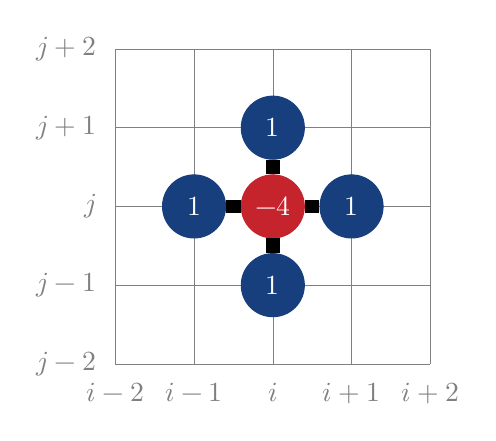
\begin{tikzpicture}
		\begin{scope}[help lines]
			\draw (-2, -2) grid (+2, +2);

			\node at (-2, -2) [label = below:$i - 2$] {};
			\node at (-1, -2) [label = below:$i - 1$] {};
			\node at ( 0, -2) [label = below:$i$]     {};
			\node at (+1, -2) [label = below:$i + 1$] {};
			\node at (+2, -2) [label = below:$i + 2$] {};

			\node at (-2, -2) [label = left:$j - 2$] {};
			\node at (-2, -1) [label = left:$j - 1$] {};
			\node at (-2,  0) [label = left:$j$]     {};
			\node at (-2, +1) [label = left:$j + 1$] {};
			\node at (-2, +2) [label = left:$j + 2$] {};
		\end{scope}

		\begin{scope}[
			every node/.style = {
				circle,
				inner sep = 0pt,
				minimum size = 0.8cm,
				text = white,
			},
		]
			\node at ( 0,  0) [draw = ETHRed,      fill = ETHRed]      (ij)   {$-4$};
			\node at (-1,  0) [draw = ETHDarkBlue, fill = ETHDarkBlue] (i-1j) {$ 1$};
			\node at (+1,  0) [draw = ETHDarkBlue, fill = ETHDarkBlue] (i+1j) {$ 1$};
			\node at ( 0, -1) [draw = ETHDarkBlue, fill = ETHDarkBlue] (ij-1) {$ 1$};
			\node at ( 0, +1) [draw = ETHDarkBlue, fill = ETHDarkBlue] (ij+1) {$ 1$};
		\end{scope}

		\draw[line width = 5pt]
			(ij) -- (i-1j)
			(ij) -- (i+1j)
			(ij) -- (ij-1)
			(ij) -- (ij+1)
		;
	\end{tikzpicture}
\end{frame}

\subsubsection*{\texorpdfstring{\texttt{inline}}{inline}}
\begin{frame}
	\frametitle{\subsubsecname}
	\begin{align*}
		\phi_{i, j, k}^{n + 1} =
			\phi_{i, j, k}^{n} &- \frac{\alpha_{4} \increment t}{(\increment x)^{2} (\increment y)^{2}} \left( \vphantom{\phi_{i, j, k}^{n}} \right. \\
				& -20 \phi_{i,     j,     k}^{n} \\
				& + 8 \phi_{i - 1, j,     k}^{n}
				  + 8 \phi_{i + 1, j,     k}^{n}
				  + 8 \phi_{i,     j - 1, k}^{n}
				  + 8 \phi_{i,     j + 1, k}^{n} \\
				& - 2 \phi_{i - 1, j - 1, k}^{n}
				  - 2 \phi_{i - 1, j + 1, k}^{n}
				  - 2 \phi_{i + 1, j - 1, k}^{n}
				  - 2 \phi_{i + 1, j + 1, k}^{n} \\
				& -   \phi_{i - 2, j,     k}^{n}
				  -   \phi_{i + 2, j,     k}^{n}
				  -   \phi_{i,     j - 2, k}^{n}
				  -   \phi_{i,     j + 2, k}^{n}
			  \left. \vphantom{\phi_{i, j, k}^{n}} \right)
	\end{align*}
	\note[item]{What do you think - which version is faster?}
\end{frame}

\begin{frame}
	\frametitle{\subsubsecname}
	\centering
	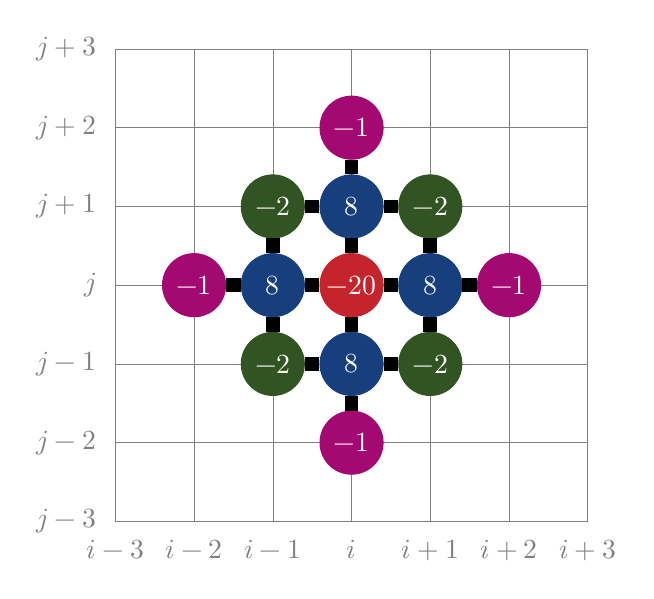
\begin{tikzpicture}
		\begin{scope}[help lines]
			\draw (-3, -3) grid (+3, +3);
			\node at (-3, -3) [label = left:$j - 3$] {};
			\node at (-3, -2) [label = left:$j - 2$] {};
			\node at (-3, -1) [label = left:$j - 1$] {};
			\node at (-3,  0) [label = left:$j    $] {};
			\node at (-3, +1) [label = left:$j + 1$] {};
			\node at (-3, +2) [label = left:$j + 2$] {};
			\node at (-3, +3) [label = left:$j + 3$] {};

			\node at (-3, -3) [label = below:$i - 3$] {};
			\node at (-2, -3) [label = below:$i - 2$] {};
			\node at (-1, -3) [label = below:$i - 1$] {};
			\node at ( 0, -3) [label = below:$i    $] {};
			\node at (+1, -3) [label = below:$i + 1$] {};
			\node at (+2, -3) [label = below:$i + 2$] {};
			\node at (+3, -3) [label = below:$i + 3$] {};
		\end{scope}

		\begin{scope}[
			every node/.style = {
				circle,
				inner sep = 0pt,
				minimum size = 0.8cm,
				text = white,
			},
		]
			\node at ( 0,  0) [draw = ETHRed,       fill = ETHRed]       (ij)     {$-20$};
			\node at (-1,  0) [draw = ETHDarkBlue,  fill = ETHDarkBlue]  (i-1j)   {$  8$};
			\node at (+1,  0) [draw = ETHDarkBlue,  fill = ETHDarkBlue]  (i+1j)   {$  8$};
			\node at ( 0, -1) [draw = ETHDarkBlue,  fill = ETHDarkBlue]  (ij-1)   {$  8$};
			\node at ( 0, +1) [draw = ETHDarkBlue,  fill = ETHDarkBlue]  (ij+1)   {$  8$};
			\node at (-1, -1) [draw = ETHDarkGreen, fill = ETHDarkGreen] (i-1j-1) {$- 2$};
			\node at (-1, +1) [draw = ETHDarkGreen, fill = ETHDarkGreen] (i-1j+1) {$- 2$};
			\node at (+1, -1) [draw = ETHDarkGreen, fill = ETHDarkGreen] (i+1j-1) {$- 2$};
			\node at (+1, +1) [draw = ETHDarkGreen, fill = ETHDarkGreen] (i+1j+1) {$- 2$};
			\node at (-2,  0) [draw = ETHMagenta,   fill = ETHMagenta]   (i-2j)   {$- 1$};
			\node at (+2,  0) [draw = ETHMagenta,   fill = ETHMagenta]   (i+2j)   {$- 1$};
			\node at ( 0, -2) [draw = ETHMagenta,   fill = ETHMagenta]   (ij-2)   {$- 1$};
			\node at ( 0, +2) [draw = ETHMagenta,   fill = ETHMagenta]   (ij+2)   {$- 1$};
		\end{scope}

		\draw[line width = 5pt]
			(ij)   -- (i-1j)
			(ij)   -- (i+1j)
			(ij)   -- (ij-1)
			(ij)   -- (ij+1)
			(i-1j) -- (i-1j-1)
			(i-1j) -- (i-1j+1)
			(i-1j) -- (i-2j)
			(i+1j) -- (i+1j-1)
			(i+1j) -- (i+1j+1)
			(i+1j) -- (i+2j)
			(ij-1) -- (i-1j-1)
			(ij-1) -- (i+1j-1)
			(ij-1) -- (ij-2)
			(ij+1) -- (i-1j+1)
			(ij+1) -- (i+1j+1)
			(ij+1) -- (ij+2)
		;
	\end{tikzpicture}
\end{frame}

\subsection*{Initial conditions}
\begin{frame}
	\frametitle{\subsecname}
	\centering
	\includegraphics[width = \textwidth, height = \textheight, keepaspectratio]{in_field}
	\par
\end{frame}

\subsection*{Result}
\begin{frame}
	\frametitle{\subsecname}
	\centering
	\includegraphics[width = \textwidth, height = \textheight, keepaspectratio]{out_field}
	\par
\end{frame}

\subsection*{Measurement setup}
\begin{frame}
	\frametitle{\subsecname}
	\begin{itemize}
		\item Fortran, C++, Rust
		\item Algorithms: \texttt{laplap}, \texttt{inline}
		\item Toolchains
			\begin{itemize}
				\item Fortran, C++: GNU, Cray, Intel, PGI
				\item Rust: \texttt{rustc}
			\end{itemize}
		\item Sequential
		\item Parallel
			\begin{itemize}
				\item Fortran, C++: OpenMP
				\item Rust: Rayon
			\end{itemize}
		\item GPU
			\begin{itemize}
				\item Fortran, C++: OpenACC, OpenMP offloading, CUDA
				\item Rust: Accel
			\end{itemize}
	\end{itemize}
	\note[item]{MPI works, but not enough time to debug the partitioner}
\end{frame}

\begin{frame}
	\frametitle{\subsecname}
	$\implies$ 84 language-compiler-algorithm combinations \\[\baselineskip]
	32 versions did not compile or run :( \\[\baselineskip]
	$\implies$ 52 versions $\times$ 4 grid sizes \\[\baselineskip]
	$\implies$ 524 measurements (1, 2, 4, 8, 12 CPU cores; GPU)
\end{frame}

\begin{frame}[fragile]
	\begin{itemize}
		\item arrays in column-major order
		\item \texttt{-O3} or equivalent
		\item no LTO
		\item optimization reports
		\item shared libraries
		\item C interface \\
			\begin{minted}{C}
				void diffuse(
					float * in_field,
					float * out_field,
					size_t  nx,
					size_t  ny,
					size_t  nz,
					size_t  num_halo,
					float   alpha,
					size_t  num_iter
				)
			\end{minted}
	\end{itemize}

	\note[item]{Show code on gitlab}
\end{frame}

\section*{Results}
\begin{frame}
	\centering
	\includegraphics[width = \textwidth, height = \textheight, keepaspectratio]{scaling_seq.png}
	\par
\end{frame}

\begin{frame}
	\centering
	\includegraphics[width = \textwidth, height = \textheight, keepaspectratio]{scaling_seq_rust.png}
	\par
\end{frame}

\begin{frame}
	\centering
	\includegraphics[width = \textwidth, height = \textheight, keepaspectratio]{scaling_cpu.png}
	\par
\end{frame}

\begin{frame}
	\centering
	\includegraphics[width = \textwidth, height = \textheight, keepaspectratio]{scaling_gpu.png}
	\par
\end{frame}

\section*{Conclusions}
\begin{frame}
	\frametitle{\secname}
	\begin{itemize}
		\item[$+$] Rust fast enough for scientific software
		\item[$+$]    Safer code
		\item[$+$]    Clearer error messages
		\item[$-$]    Support for certain features is lacking
		\item[$\sim$] All languages sometimes lead to lots of boilerplate
	\end{itemize}

	\note[item]{Rust compiler does good job of vectorizing code}
	\note[item]{Rust: clear what you get}
	\note[item]{Fortran/C++: different support, many bugs}
	\note[item]{GNU doesn't warn about lack of offloading}
	\note[item]{Cray sometimes silently generates invalid PTX code}
\end{frame}

\subsection*{Recommendations}
\begin{frame}
	\frametitle{\subsecname}
	\begin{itemize}
		\item in 2020
			\begin{itemize}
				\item Rust for frontend/driver
			\end{itemize}
		\item hopes for after 2020
			\begin{itemize}
				\item GPU support
				\item Evolve \texttt{ndarray}
				\item ScaLAPACK bindings, \textellipsis
			\end{itemize}
		\item $\implies$ continue to pursue Rust in HPC
			\begin{itemize}
				\item it has potential
			\end{itemize}
	\end{itemize}

	See:
	\begin{itemize}
		\item \url{https://www.arewelearningyet.com/scientific-computing/}
		\item \url{https://www.arewelearningyet.com/gpu-computing/}
	\end{itemize}

	\note[item]{With Cray and Intel moving to LLVM, cross-language LTO soon?}
\end{frame}

\section*{Two years later …}
\begin{frame}[c]
	\centering
	\textbf{\Large \secname}
\end{frame}

\begin{frame}[c]
	\centering
	\textbf{\Large not much has changed :(}
\end{frame}

\begin{frame}
	\frametitle{\secname}
	\begin{itemize}
		\item \texttt{cargo-cmake} \textrightarrow{} \href{https://github.com/corrosion-rs/corrosion}{\texttt{corrosion}}
		\item \href{https://github.com/rust-cuda}{\texttt{rust-cuda}} \textrightarrow{} \href{https://github.com/Rust-GPU/}{\texttt{rust-gpu}}
		\item \texttt{nvptx64-nvidia-cuda} still a Tier 2 target
	\end{itemize}
\end{frame}

\section*{Questions?}
\begin{frame}
	\frametitle{\secname}
	\includegraphics[width = \textwidth, height = \textheight, keepaspectratio]{rustacean-flat-gesture.png}
\end{frame}

\section*{Keep in touch?}
\begin{frame}
	\frametitle{\secname}

	\begin{itemize}
		\item \href{mailto:michal@sudwoj.name}{\texttt{michal@sudwoj.name}}
		\item \url{https://github.com/westernmagic/rust-in-hpc}
		\item \url{www.linkedin.com/in/michalsudwoj}
	\end{itemize}
\end{frame}

\cscsthankyou{Thank you for you attention}

\end{document}
